% Hlavicka pro protokoly z fyzikalniho praktika.
% Verze pro: LaTeX
% Verze hlavicky: 22. 2. 2007
% Autor: Ustav fyziky kondenzovanych latek
% Ke stazeni: www.physics.muni.cz/ufkl/Vyuka/
% Licence: volne k pouziti, nejlepe k vcasnemu odevzdani protokolu z Vaseho mereni.


\documentclass[czech,11pt,a4paper]{article}
\usepackage[T1]{fontenc}
\usepackage{graphicx}
\usepackage{mathtools}
\usepackage{amssymb}
\usepackage{amsthm}
\usepackage{thmtools}
\usepackage{xcolor}
\usepackage{nameref}
\usepackage{babel}
\usepackage{hyperref}
\usepackage{multicol}
\usepackage[export]{adjustbox}
\usepackage{subcaption}
\usepackage{caption}
\usepackage{multirow}
\usepackage{float}
\usepackage{placeins}




%%% Nemente:
\usepackage[margin=2cm]{geometry}
\newtoks\jmenopraktika \newtoks\jmeno \newtoks\datum
\newtoks\obor \newtoks\skupina \newtoks\rocnik \newtoks\semestr
\newtoks\cisloulohy \newtoks\jmenoulohy
\newtoks\tlak \newtoks\teplota \newtoks\vlhkost
%%% Nemente - konec.


%%%%%%%%%%% Doplnte pozadovane polozky:

\jmenopraktika={Fyzikální praktikum 2}  % nahradte jmenem vaseho predmetu
\jmeno={Teodor Duraković}            % nahradte jmenem mericiho
\datum={24.~září 2024}        % nahradte datem mereni ulohy
\obor={F}                     % nahradte zkratkou vami studovaneho oboru
\skupina={Po 14:00}            % nahradte dobou vyuky vasi seminarni skupiny
\rocnik={II}                  % nahradte rocnikem, ve kterem studujete
\semestr={III}                 % nahradte semestrem, ve kterem studujete

\cisloulohy={1}               % nahradte cislem merene ulohy
\jmenoulohy={Studium elektromagnetické indukce} % nahradte jmenem merene ulohy

\tlak={1\, 008}                   % nahradte tlakem pri mereni (v hPa)
\teplota={20.3}               % nahradte teplotou pri mereni (ve stupnich Celsia)
\vlhkost={42}               % nahradte vlhkosti vzduchu pri mereni (v %)

%%%%%%%%%%% Konec pozadovanych polozek.


%%%%%%%%%%% Uzitecne balicky:

%%%%%% Zamezeni parchantu:
\widowpenalty 10000 \clubpenalty 10000 \displaywidowpenalty 10000
%%%%%% Parametry pro moznost vsazeni vetsiho poctu obrazku na stranku
\setcounter{topnumber}{3}	  % max. pocet floatu nahore (specifikace t)
\setcounter{bottomnumber}{3}	  % max. pocet floatu dole (specifikace b)
\setcounter{totalnumber}{6}	  % max. pocet floatu na strance celkem
\renewcommand\topfraction{0.9}	  % max podil stranky pro floaty nahore
\renewcommand\bottomfraction{0.9} % max podil stranky pro floaty dole
\renewcommand\textfraction{0.1}	  % min podil stranky, ktery musi obsahovat text
\intextsep=8mm \textfloatsep=8mm  %\intextsep pro ulozeni [h] floatu a \textfloatsep pro [b] or [t]

% Tecky za cisly sekci:
\renewcommand{\thesection}{\arabic{section}.}
\renewcommand{\thesubsection}{\thesection\arabic{subsection}.}
\renewcommand{\thesubsubsection}{\thesubsection\arabic{subsubsection}.}
% Jednopismenna mezera mezi cislem a nazvem kapitoly:
\makeatletter \def\@seccntformat#1{\csname the#1\endcsname\hspace{1ex}} \makeatother


%%%%%%%%%%%%%%%%%%%%%%%%%%%%%%%%%%%%%%%%%%%%%%%%%%%%%%%%%%%%%%%%%%%%%%%%%%%%%%%
%%%%%%%%%%%%%%%%%%%%%%%%%%%%%%%%%%%%%%%%%%%%%%%%%%%%%%%%%%%%%%%%%%%%%%%%%%%%%%%
% Zacatek dokumentu
%%%%%%%%%%%%%%%%%%%%%%%%%%%%%%%%%%%%%%%%%%%%%%%%%%%%%%%%%%%%%%%%%%%%%%%%%%%%%%%
%%%%%%%%%%%%%%%%%%%%%%%%%%%%%%%%%%%%%%%%%%%%%%%%%%%%%%%%%%%%%%%%%%%%%%%%%%%%%%%

\begin{document}
	
	%%%%%%%%%%%%%%%%%%%%%%%%%%%%%%%%%%%%%%%%%%%%%%%%%%%%%%%%%%%%%%%%%%%%%%%%%%%%%%%
	% Nemente:
	%%%%%%%%%%%%%%%%%%%%%%%%%%%%%%%%%%%%%%%%%%%%%%%%%%%%%%%%%%%%%%%%%%%%%%%%%%%%%%%
	\thispagestyle{empty}
	
	{
		\begin{center}
			\sf 
			{\Large Ústav fyzikální elektroniky Přírodovědecké fakulty Masarykovy univerzity} \\
			\bigskip
			{\huge \bfseries FYZIKÁLNÍ PRAKTIKUM} \\
			\bigskip
			{\Large \the\jmenopraktika}
		\end{center}
		
		\bigskip
		
		\sf
		\noindent
		\setlength{\arrayrulewidth}{1pt}
		\begin{tabular*}{\textwidth}{@{\extracolsep{\fill}} l l}
			\large {\bfseries Zpracoval:}  \the\jmeno & \large  {\bfseries Naměřeno:} \the\datum\\[2mm]
			\large  {\bfseries Obor:} \the\obor  \hspace{40mm}  {\bfseries Skupina:} \the\skupina %
			%{\bfseries Ročník:} \the\rocnik \hspace{5mm} {\bfseries Semestr:} \the\semestr  
			&\large {\bfseries Testováno:}\\
			\\
			\hline
		\end{tabular*}
	}
	
	\bigskip
	
	{
		\sf
		\noindent \begin{tabular}{p{3cm} p{0.6\textwidth}}
			\Large  Úloha č. {\bfseries \the\cisloulohy:} \par
			\smallskip
			$T=\the\teplota$~$^\circ$C \par
			$p=\the\tlak$~hPa \par
			$\varphi=\the\vlhkost$~\%
			&\Large \bfseries \the\jmenoulohy  \\[2mm]
		\end{tabular}
	}
	
	\vskip1cm
	
	%%%%%%%%%%%%%%%%%%%%%%%%%%%%%%%%%%%%%%%%%%%%%%%%%%%%%%%%%%%%%%%%%%%%%%%%%%%%%%%
	% konec Nemente.
	%%%%%%%%%%%%%%%%%%%%%%%%%%%%%%%%%%%%%%%%%%%%%%%%%%%%%%%%%%%%%%%%%%%%%%%%%%%%%%%
	
	%%%%%%%%%%%%%%%%%%%%%%%%%%%%%%%%%%%%%%%%%%%%%%%%%%%%%%%%%%%%%%%%%%%%%%%%%%%%%%%
	%%%%%%%%%%%%%%%%%%%%%%%%%%%%%%%%%%%%%%%%%%%%%%%%%%%%%%%%%%%%%%%%%%%%%%%%%%%%%%%
	% Zacatek textu vlastniho protokolu
	%%%%%%%%%%%%%%%%%%%%%%%%%%%%%%%%%%%%%%%%%%%%%%%%%%%%%%%%%%%%%%%%%%%%%%%%%%%%%%%
	%%%%%%%%%%%%%%%%%%%%%%%%%%%%%%%%%%%%%%%%%%%%%%%%%%%%%%%%%%%%%%%%%%%%%%%%%%%%%%%
	

	\section{Zadání}
	\textbf{Závislost indukovaných pulsů na výchylce}	\\
	1. Změřit závislost amplitudy a šířky napěťového pulsu indukovaného v cívce na úhlové amplitudě kmitů, zjistit, zda je amplituda napětí $U_{max}$ skutečně úměrná amplitudě úhlu $\theta_{max}$ , a čas $\Delta t$\ úhlu úměrný nepřímo.\\
	2. Spolu s naměřenými hodnotami do grafu vynést i přímku odpovídající modelové lineární závislosti.\\
	3. Určit efektivní poloměr použité cívky a odhadnout magnetický dipólový moment použitého magnetu.\\
	\textbf{Tlumení pohybu magnetu}\\
	1. Zjistit průběh tlumení kmitavého pohybu v závislosti na zatěžovacím odporu R.\\
	2. Ověřit, že je pokles v případě dominantního elektromagnetického tlumení lineární a směrnice $\alpha$ je nepřímo úměrná $R+R_c$\\
	3. Stanovit koeficient útlumu pro případ převládajícího mechanického tlumení.\\
	
	\section{Postup, metody měření}
	\subsection{Závislost indukovaných pulsů na výchylce}
	Základním pilířem tohoto praktika je Faradayův zákon:
	\begin{equation}
		U = - \frac{d \Phi}{dt}
	\end{equation}
	ten vyjadřuje vztah mezi napětím $U$ indukovaným v uzavřené smyčce a časovou změnou magnetického toku $\Phi$ procházejícího plochou smyčky.
	Magnetické pole tvořené magnetem s dipólovým momentem $m$~je dáno vztahem
	\begin{equation}
		\boldsymbol{B}(\boldsymbol{r})=\frac{\mu_0}{4 \pi r^3}\left[\frac{3(\boldsymbol{r} \cdot \boldsymbol{m}) \boldsymbol{r}}{r^2}-\boldsymbol{m}\right],
	\end{equation}
	kde $\boldsymbol{r}$ je polohový vektor vztažený na magnetický dipól, $m$ je magnetický dipólový moment a $\mu_0$ je permeabilita vakua. Magnetický indukční tok pole magnetického dipólu je roven
	\begin{equation}
		\Phi(x)=\int_S \boldsymbol{B} \mathrm{~d} \boldsymbol{S}=\frac{\mu_0 m}{2} \frac{a^2}{\left(a^2+x^2\right)^{3 / 2}},
	\end{equation}
	kde $ a$ je poloměr kruhového závitu, do jehož středu umístíme počátek osy $x$. \\
	K určení napětí indukovaného na smyčce užijeme Faradayův zákon (1). Nechť v čase $t = 0$ prochází dipól středem cívky, pak je jeho souřadnice $x$ vyjádřena vztahem $x = v_{max}t$. Provedeme-li za tohoto předpokladu časovou derivaci magnetického indukčního toku $\Phi$, získáme pro napětí indukované v cívce s $N$ závity:
	\begin{equation}
		U(t)=-N \frac{\mathrm{~d} \Phi}{\mathrm{~d} t}=\frac{3 N \mu_0 m v_{\max }}{2 a^2} \frac{v_{\max } t / a}{\left[1+\left(v_{\max } t / a\right)^2\right]^{5 / 2}}.
	\end{equation}
	Časový průběh indukovaného napětí bude při průletu magnetu vypadat přibližně takto:
		\begin{figure}[h]
	\begin{center}
			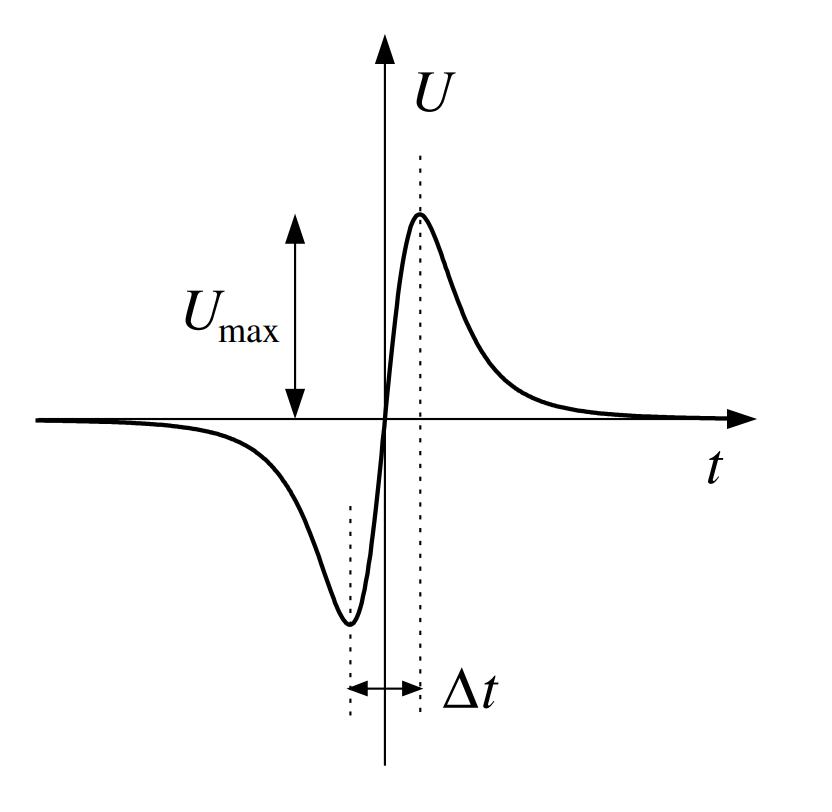
\includegraphics[width=0.4\linewidth]{prubeh}
	\end{center}
	\end{figure}
	Křivka závislosti obsahuje jedno maximum a jedno minimum, které nám umožní zavést šířku pulsu $\Delta t$ jako časový rozdíl mezi okamžikem maximálního a minimálního napětí a amplitudu napěťového pulsu $U_{max}$. Je-li indukované napětí popsáno rovnicí (4), nalezneme minimum napětí v bodě $t_{min} = - \frac{a}{2v_{max}}$ a maximum v bodě  $t_{max} =  \frac{a}{2v_{max}}$. \textbf{Šířka pulsu je tedy nepřímo úměrná rychlosti průletu:}
	\begin{equation}
		\Delta t = a v^{-1}_{max}.
	\end{equation}
	Dále můžeme určit amplitudu napětí
	\begin{equation}
		U_{\max }=\frac{24}{25 \sqrt{5}} \frac{N \mu_0 m}{a^2} v_{\max },
	\end{equation}
	která je naopak, jak je ze vztahu patrno, rychlosti průletu \textbf{přímo úměrná}.
	Rychlost $v_{max}$ lze určit ze zákona zachování energie. Je-li hmotnost magnetu spolu s nosníkem rovna $M$, platí
	\begin{equation}
		\frac{1}{2} M v_{\max }^2=M g L\left(1-\cos \theta_{\max }\right),
	\end{equation}
	kde $g$ je zemské tíhové zrychlení, $L$ délka kyvadla a $\theta_{max}$ úhlová amplituda jeho kmitů. \\
	Amplitudu rychlosti tedy získáme prostřednictvím vztahu
	\begin{equation}
		v_{\max }=2 \sqrt{g L} \sin \left(\frac{\vartheta_{\max }}{2}\right) \approx \sqrt{g L} \vartheta_{\max }.
	\end{equation}
	
	
	\subsection{Tlumení pohybu magnetu}
	V předchozí části jsme o tlumení kmitavého pohybu neuvažovali. Při analýze více kmitů (nikoli pouze prvního průletu, jako v předchozí části) bude pohyb tlumený mechanicky (odporem vzduchu) a elektromagneticky.
	Pokles amplitudy mechanicky tlumeného napětí lze popsat vztahem 
	\begin{equation}
		U _{\max}(t) = U_{\max}(0) e^{-\beta t} ,
	\end{equation}
	kde $U_{\max}$ je počáteční amplituda napětí a $\beta$ koeficient tlumení.

	Při čistě elektromagnetickém tlumení je pohyb magnetu tlumen magnetickým polem cívky, které vzniká kvůli indukovanému napětí. Proud vyvolaný indukovaným napětím je v souladu s Ohmovým zákonem $ R = U/I$ závislý na odporu celého obvodu, přičemž se tento odpor skládá z vlastního odporu cívky $R_c$ a zatěžovacího odporu $R$. 
	
	Lze uvažovat, že vzniklý proud bude podléhat závislosti $I = U/R_{celk.} = U / (R+R_c)$, s rostoucím zatěžovacím odporem bude tedy buzený proud klesat a spolu s ním bude klesat i míra tlumení, jelikož je velikost magnetické indukce dle Biot-Savartova zákona přímo úměrná proudu ($B = \frac {\mu_0 N I}{2R}  $).
	
	Pro elektromagnetické tlumení bude pokles amplitudy kmitů \textbf{lineární}:
	\begin{equation}
		U_{\max} (t) = U_{\max}(0) - \alpha t
	\end{equation}
	
	
	
	\section{Měření}
	\subsection{Závislost indukovaných pulsů na výchylce}
	Známé údaje pro kalkulaci hledaných hodnot jsou:\\
	$L = 1.7 \,\mathrm{m}, \,\, g = 9.81 \rm{m.s^{-2}}, \,\, N = 1000 $\\
	Po zpracování naměřených dat získáme hodnoty \\
	\begin{center}
		$
	\begin{array}{|c|c|c|c|}
		\hline \theta_{\max} [^\circ]& U_{\max}[\mathrm{V}] & \Delta t [\mathrm{s}] & v_{\max}[\rm{m/s}] \\
		\hline 2 & 0.045 & 0.086 & 0.14 \\
		\hline 3 & 0.088 & 0.050 & 0.21 \\
		\hline 4 & 0.11 & 0.036 & 0.29 \\
		\hline 5 & 0.14 & 0.032 & 0.36 \\
		\hline 6 & 0.18 & 0.024 & 0.43 \\
		\hline 7 & 0.21 & 0.021 & 0.50 \\
		\hline 8 & 0.24 & 0.018 & 0.57 \\
		\hline 9 & 0.27 & 0.016 & 0.64\\
		\hline 10 & 0.30 & 0.014 & 0.71 \\
		\hline 11 & 0.34 & 0.013 & 0.78 \\
		\hline 12 & 0.36 & 0.012 & 0.86 \\
		\hline
	\end{array}$
	\end{center}
	Z čehož vykreslíme závislosti amplitudy napětí $U_{\max}$ na amplitudě výchylky $\theta_{\max}$ a závislost šířky napěťového pulsu na amplitudě výchylky:
	 \begin{figure}[H]
		\begin{subfigure}{0.5\textwidth}
			\includegraphics[width=0.9\linewidth, ]{napetivychylka} 
		\end{subfigure}
		\begin{subfigure}{0.5\textwidth}
			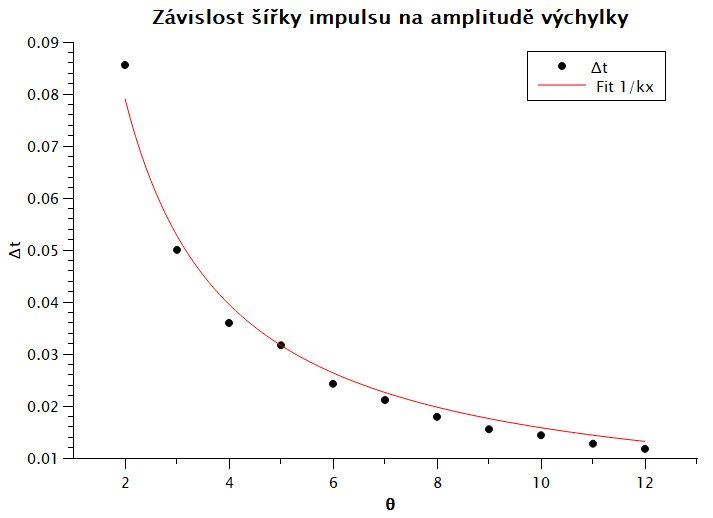
\includegraphics[width=0.9\linewidth, ]{impulsvychylka}
		\end{subfigure} \end{figure}
	Vidíme, že je amplituda napětí skutečně přímo úměrná amplitudě výchylky, zatímco šířka impulsu (a tedy i rychlost) je výchylce úměrná nepřímo.\\
	
	Poloměr cívky určíme pomocí formule (5). Po vykreslení závislosti časového impulsu na amplitudě výchylky fitujeme křivku $\frac{k}{v}$, získané $k$ bude odpovídat poloměru cívky. 
	
	 \begin{figure}[H]
		\begin{subfigure}{0.5\textwidth}
			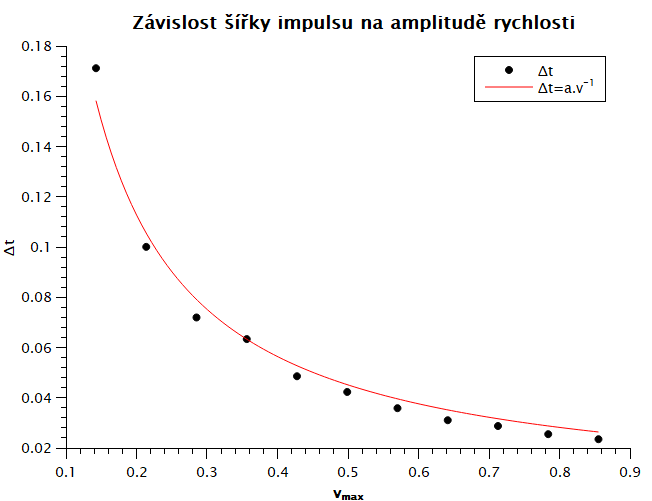
\includegraphics[width=0.9\linewidth, ]{impulsrychlost} 
		\end{subfigure}
		\begin{subfigure}{0.5\textwidth}
				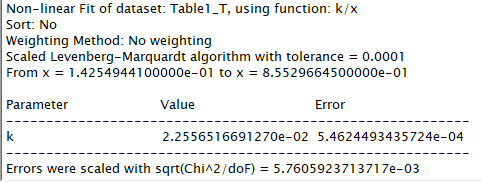
\includegraphics[width=0.9\linewidth, ]{vysledkyfitu}				
				\caption{výsledek fitování křivky k/v}
	\end{subfigure} \end{figure}
    Pro poloměr cívky získáváme hodnotu $ a = 22.6 \pm 0.05 \,\rm mm$, což odpovídá odhadované hodnotě, poloměr jsme však jinými metodami neměřili.\\
    Magnetický dipólový moment vypočteme pomocí formule (6), přičemž všechny členy kromě amplitudy napětí a rychlosti položíme rovny konstantě úměrnosti $k$. 
    \begin{gather}
    	k =\frac{24}{25 \sqrt{5}} \frac{N \mu_0 m}{a^2} ,\\
    	U_{\max }= k v_{\max }
    \end{gather}	
    Konstantu $k$ získáme lineárním fitem $(U=kv)$ závislosti amplitudy napětí na amplitudě rychlosti. Získáváme
    \begin{equation*}
    	k = 0.42 \pm 0.004 \,\rm \frac{V}{^\circ},
    \end{equation*}
    další úpravou formule (11) vyjádříme magnetický dipólový moment, získáváme hodnotu\\ $m = 0.396 \pm 0.02 \,\rm A.m^2$
    
   \subsection{Tlumení pohybu magnetu}
   Analyzujeme tlumení pohybu v závislosti na velikosti zatěžovacího odporu $R$, měření provádíme pro hodnoty zatěžovacích odporů $R = \{1\mathrm{M} \Omega, 1\mathrm{k}\Omega, 200\Omega, 150\Omega, 120\Omega, 100\Omega, 80\Omega, 60\Omega, 40\Omega, 20\Omega \}$. V souladu s výše uvedenými předpoklady při velkých zatěžovacích odporech převládá tlumení mechanické, exponenciální, zatímco při menších odporech převládá tlumení elektromagnetické, lineární:
    \begin{figure}[H]
   	\begin{subfigure}{0.33\textwidth}
   		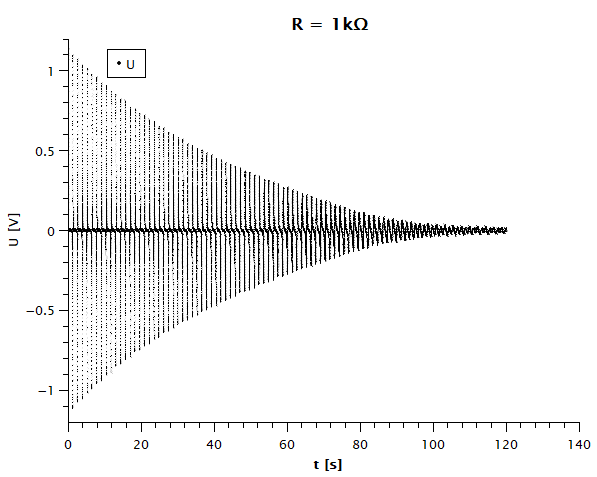
\includegraphics[width=0.9\linewidth, ]{r1k} 
   	\end{subfigure}
   	\begin{subfigure}{0.33\textwidth}
   			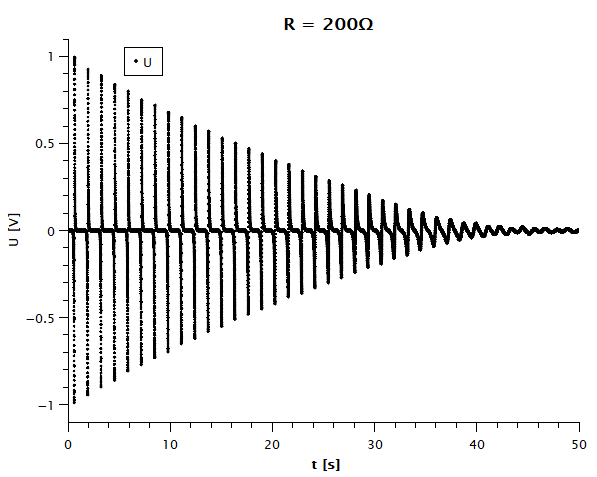
\includegraphics[width=0.9\linewidth, ]{r200} 
   	\end{subfigure}
   	\begin{subfigure}{0.33\textwidth}
   			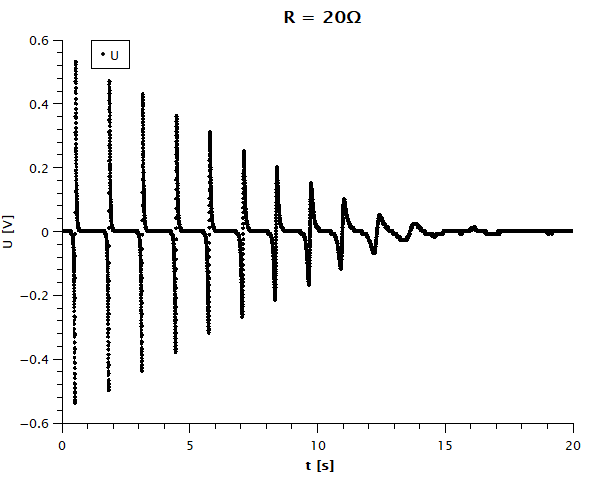
\includegraphics[width=0.9\linewidth, ]{r20}				
   		
   \end{subfigure}	\caption{průběh indukovaného napětí při zatěžovacích odporech 1k$\Omega$, 200$\Omega$ a 20$\Omega$} \end{figure}
	Jak již zmiňuje formule (9), u převládajícího mechanického tlumení se jeho průběh bude odvíjet od hodnoty koeficientu tlumení $\beta$. Jeho hodnotu pro odpory $R = 1\mathrm{M}\Omega, 1\mathrm{k}\Omega$ zjistíme fitem funkce odpovídající formuli (9):
	
	\begin{figure}[H]
		\begin{subfigure}{0.5\textwidth}
			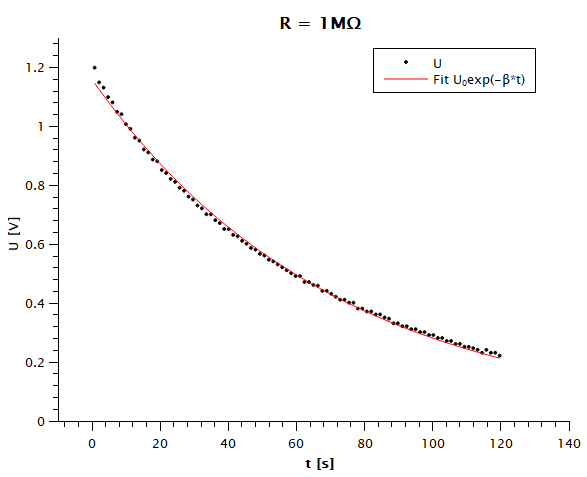
\includegraphics[width=0.9\linewidth, ]{tlumeni1m} 
		\end{subfigure}
		\begin{subfigure}{0.5\textwidth}
			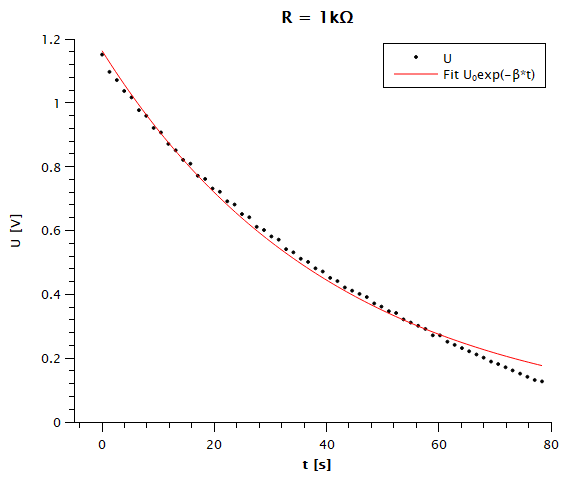
\includegraphics[width=0.9\linewidth, ]{tlumeni1k}		
	\end{subfigure} \end{figure} 
	Pro jednotlivé odpory získáváme koeficienty:
	\begin{equation*}
		\beta_{1\mathrm{M}\Omega} = 0.01415 \pm 0.00007\,\mathrm{s}^{-1}, \,\,\,\, \beta_{1\mathrm{k}\Omega} = 0.02405 \pm 0.0003\,\mathrm{s}^{-1}
	\end{equation*}
	Zatímco pro odpor $R = 1\mathrm{M}\Omega$ je tato aproximace poměrně přesná, u odporu $R = 1 \mathrm{k}\Omega$ již pozorujeme viditelnou deviaci od skutečných hodnot, působení elektromagnetického tlumení je pro tento odpor již nezanedbatelné.
	
	Při menších odporech je tlumení převážně elektromagnetické, lineární. Při analýze dat je však nutné uvažovat, že měřená amplituda je ovlivněna úbytkem napětí na zatěžovacím odporu. Skutečné indukované napětí získáme užitím formule $U_M = \frac{R_c+R}{R}U$. Hodnota odporu cívky je dána: $R_c = 40 \,\rm \Omega$ Po úpravě hodnot lineárně aproximujeme průběhy pro jednotlivé odpory, z čehož získáme koeficient lineárního útlumu $\alpha$. Získáváme:
	
   \begin{figure}[h]
   \begin{center}
   	
   			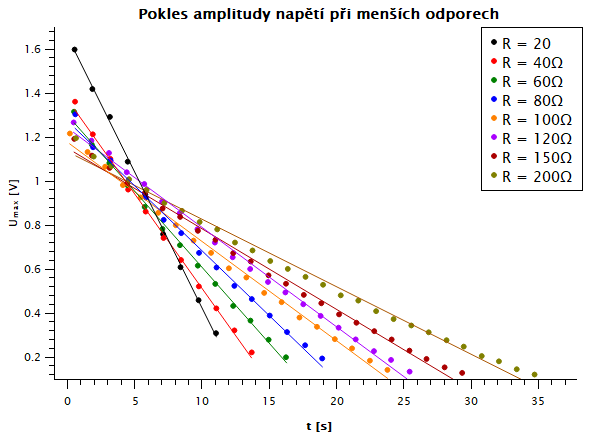
\includegraphics[width=0.6\linewidth, ]{tlumeniostatni} 
   \end{center}
   		
    \end{figure} 
    \begin{center}
    		$\begin{array}{l|c}
    	R [\Omega] & \alpha  \, [\mathrm{V.s}^{-1}]           \\ \hline
    	20         & -0.1234 \pm 0.0016  \\ \hline
    	40         & -0.0858 \pm 0.0014  \\ \hline
    	60         & -0.0691\pm 0.0012   \\ \hline
    	80         & -0.0590 \pm -0.0011 \\ \hline
    	100        & -0.0451\pm 0.0007   \\ \hline
    	120        & -0.0451\pm 0.0007  \\ \hline
    	150        & -0.0366 \pm 0.0006  \\ \hline
    	200        & -0.0307\pm 0.0006  
    \end{array}$
    \end{center}
    K ověření nepřímé úměrnosti koeficientu tlumení na celkovém odporu vykreslíme závislost záporu jeho převrácené hodnoty na zatěžovacím odporu:
    
    \begin{figure}[h]
    	\begin{center}
    		
    		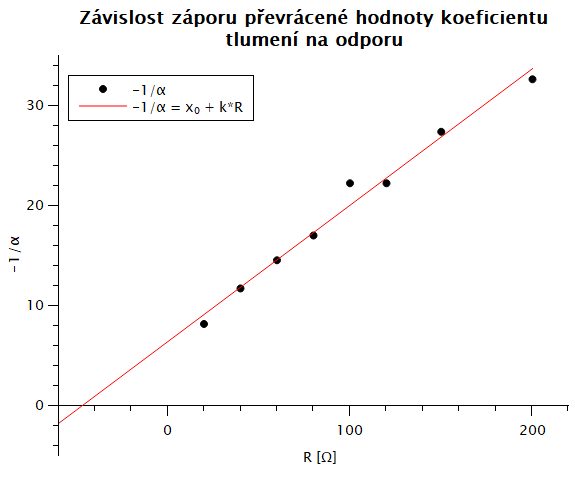
\includegraphics[width=0.4\linewidth, ]{koefodpor} 
    	\end{center}
    	\end{figure}
   	Pokud bychom koeficient tlumení neuvažovali v závislosti na zatěžovacím odporu, ale na odporu celkovém, průsečík osy $R$ by se přibližně nacházel v počátku soustavy souřadnic. V případě uvedeném výše by se však měl nacházet v bodě $R = -R_c$, což lze ověřit řešením rovnice $0 = x_0 + kR$. Získáváme $R = -46 \pm 6 \,\rm \Omega$, což je odporu cívky $R_c$ velmi blízké. Koeficient tlumení je tedy skutečně nepřímo úměrný celkovému odporu obvodu.
	\section{Závěr}
	Experimentálně se nám podařilo ověřit veškeré závislosti a získat požadované hodnoty. Experimentální výsledky potvrdily teoretické předpoklady, přičemž nám k tomuto ověření chyby měření zásadně nebránily.
	
	
	\section{Použitý kód}
	{\tiny \begin{verbatim}
	import numpy as np
	from uncertainties import ufloat
	
	k = ufloat(0.42, 0.004)  
	a = ufloat(0.02255,0.000546)
	N = ufloat (1000, 0)
	mu = ufloat(1.256637e-6,0)
	m = (k*a**2*25*np.sqrt(5))/(N*mu*24)
	print (m)
	
	y0 = ufloat(  6.2860368129097e+00 , 7.8935730298951e-01 )  
	k = ufloat(1.3653338376198e-01 ,  7.0993809199494e-03   )
	x0 = (-y0/k)
	print (x0)
	\end{verbatim}}

	

	
	% Nakonec nezapomeňte projet text programem vlna nebo vlnka, např.
	% 	vlna -m -l -n mojeuloha.tex
	% nebo zkontrolovat a opravit jednopísmenné předložky na koncích řádků ručně.
	
\end{document}
